\documentclass[tikz,border=10pt]{standalone}
\begin{document}
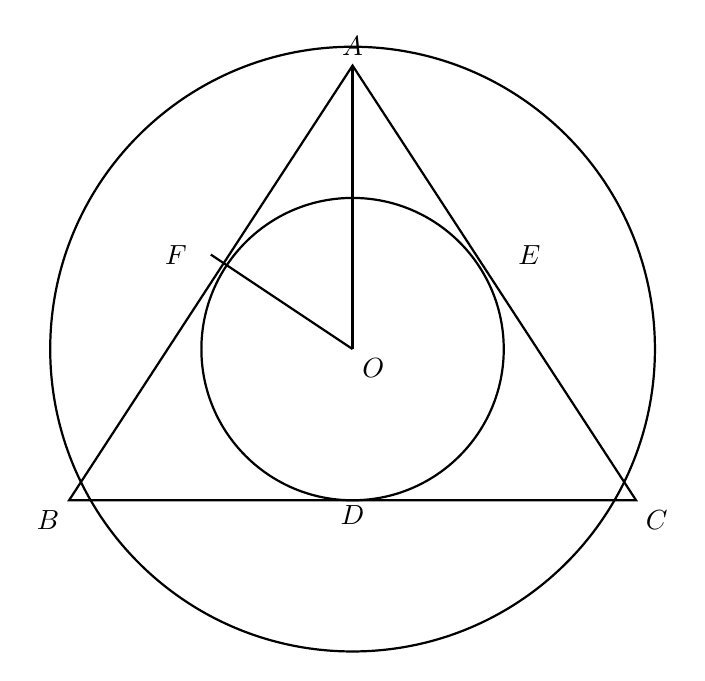
\begin{tikzpicture}[scale=1.2]
\coordinate (O) at (0,0);
\coordinate (A) at (0,3);
\coordinate (B) at (-3,-1.6);
\coordinate (C) at (3,-1.6);
\coordinate (D) at (0,-1.55);
\coordinate (E) at (1.5,1.0);
\coordinate (F) at (-1.5,1.0);

\draw[thick] (O) circle (3.2);
\draw[thick] (O) circle (1.6);
\draw[thick] (A) -- (B) -- (C) -- cycle;
\draw[thick] (A) -- (O);
\draw[thick] (O) -- (F);

\node[above] at (A) {$A$};
\node[below left] at (B) {$B$};
\node[below right] at (C) {$C$};
\node[below] at (D) {$D$};
\node[right] at (1.65,1.0) {$E$};
\node[left] at (-1.65,1.0) {$F$};
\node[below right] at (O) {$O$};
\end{tikzpicture}
\end{document}
